% title page
\frame{
   \begin{center}
    \huge{子どもIT未来塾 第5回}\\

    \vspace{34pt}
	   {\huge Raspberry Piをリモコンにしてみよう}\\
    \vspace{24pt}
    \large{奥山 祐市}\\
    \vspace{10pt}
    \large{\the\year 年 8月24日}
  \end{center}
}

% \begin{frame}[fragile]
%     \frametitle{教材のアップデートをしよう}
%     \begin{center}
%         \begin{columns}
%             \begin{column}{0.48\textwidth}
%                 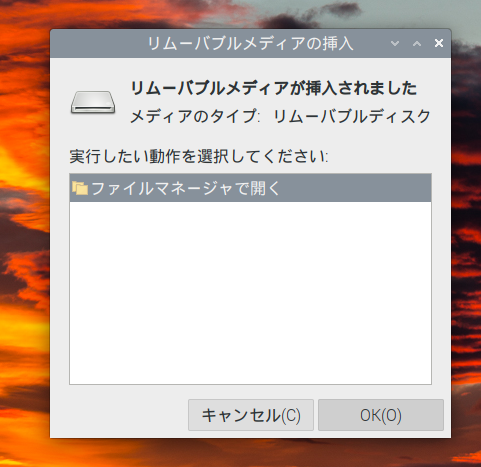
\includegraphics[width=\textwidth]{images/slide/insert_removal_media.png}
%             \end{column}
%             \begin{column}{0.48\textwidth}
%                 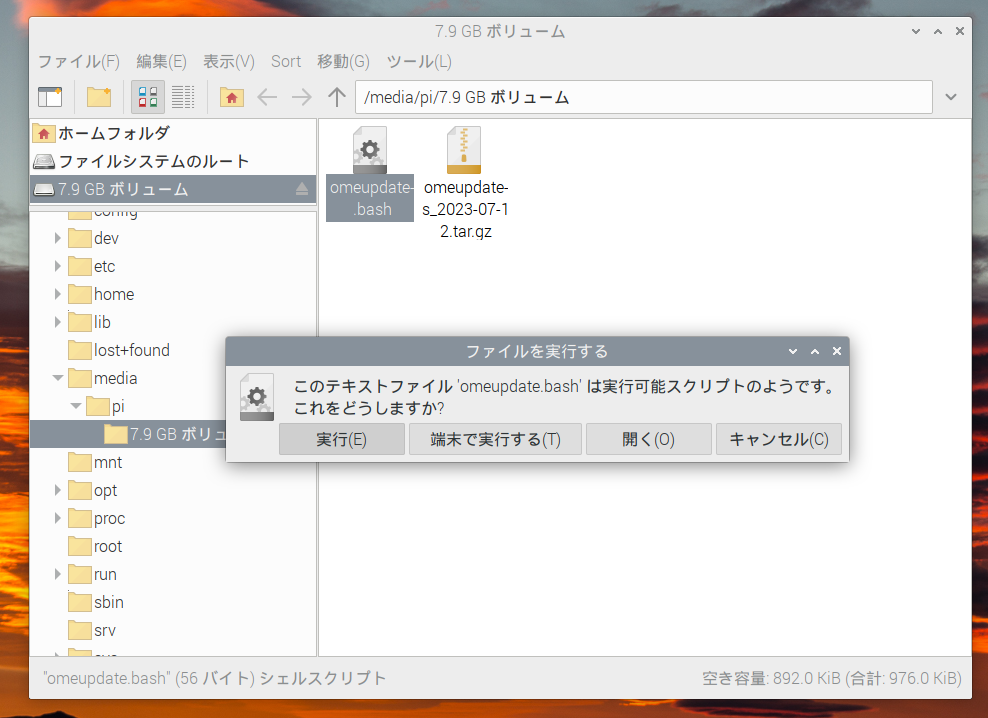
\includegraphics[width=\textwidth]{images/slide/exe_volume.png}
%             \end{column}
%         \end{columns}
%         {USBメモリをラズパイにさして、教材をアップデートするプログラムを実行しよう}
%     \end{center}
% \end{frame}

\begin{frame}[fragile]
    \frametitle{使うディレクトリをコピーしよう}
    \begin{itemize}
        \item コピーコマンドを実行しよう
    \end{itemize}
    \vspace{10pt}
    \begin{lstlisting}[title=ディレクトリのコピー,label=workfilecopy]
    <#green#pi@raspberrypi#>:<#blue#~ $#> cp -r /usr/local/share/ome/05 ~
    <#green#pi@raspberrypi#>:<#blue#~ $#>
    \end{lstlisting}
\end{frame}

\begin{frame}[fragile]
    \frametitle{目次}
    \begin{enumerate}
        \item センサーについて知ろう
        \item FaBoのセンサーを使ってみよう
        \item 赤外線について知ろう
        \item 赤外線を送信・受信してみよう
        \item 赤外線を使って家電を動かしてみよう
        \item 演習とコマンドの続き
    \end{enumerate}
\end{frame}
